\documentclass[12pt,a4paper]{article}

\usepackage[utf8]{inputenc}
\usepackage[T1]{fontenc}
\usepackage[margin=2.5cm]{geometry}
\usepackage{amsmath}
\usepackage{booktabs}
\usepackage{graphicx}
\usepackage{xcolor}
\usepackage[hidelinks]{hyperref}
\renewcommand{\thesubsubsection}{%
\ifnum\value{subsection}>0\relax\thesubsection.\arabic{subsubsection}%
\else\thesection.\arabic{subsubsection}\fi}

\title{Project 1\\SDSS: Spectral Analysis}
\author{Cserpák Mihály Márkó\\Neptun ID: AD0FHH}
\date{}

\begin{document}

\maketitle

\section{Gathering Data}

I obtained the data from Sloan Digital Sky Survey (SDSS) Data Release 17 through SkyServer.\footnote{SDSS Data Release 17: \url{https://www.sdss4.org/dr17/}.} The four variables I want to predict are redshift and the magnitudes in the $g$, $r$, and $i$ bands (\texttt{cModelMag\_g}, \texttt{cModelMag\_r}, and \texttt{cModelMag\_i}). Based on ChatGPT's recommendation, I chose a sample of 5,000 galaxies for training. These galaxies were selected to have valid values for all four prediction targets.

\section{Understanding the Data}

I loaded the spectra from FITS files into pandas DataFrames, which store data in rows and columns.\footnote{pandas DataFrame documentation: \url{https://pandas.pydata.org/docs/reference/api/pandas.DataFrame.html}.} Each row corresponds to one spectral pixel. SDSS stores the flux, logarithmic wavelength, inverse variance, and quality masks for each pixel.\footnote{SDSS optical spectra and uncertainty documentation: \url{https://www.sdss4.org/dr17/spectro/spectro_basics/}.} Tables~\ref{tab:spectrum-one} and~\ref{tab:spectrum-two} show the first four and last four pixels of two galaxies.

The \texttt{loglam} value is the base-10 logarithm of the wavelength expressed in angstroms:
\begin{equation}
    \mathrm{loglam}_i = \log_{10}\!\left(\frac{\lambda_i}{1\,\text{\AA}}\right).
\end{equation}
The wavelength is recovered as
\begin{equation}
    \lambda_i = 10^{\mathrm{loglam}_i}\,\text{\AA}.
\end{equation}
I appended the wavelength column to the tables. The flux values are the inputs on which I will train the models.

Each \texttt{loglam} value specifies the centre of a spectral pixel in logarithmic wavelength. The spectra use the same logarithmic step size, although their starting and ending wavelengths differ. To select a wavelength range shared by all 5,000 galaxies, I will take the largest starting wavelength and the smallest ending wavelength. The flux values at matching wavelength centres within this range will form the model inputs.
 Figure~\ref{fig:example-galaxy-spectra} shows examples of the downloaded galaxy spectra.

\begin{figure}[htbp]
\centering
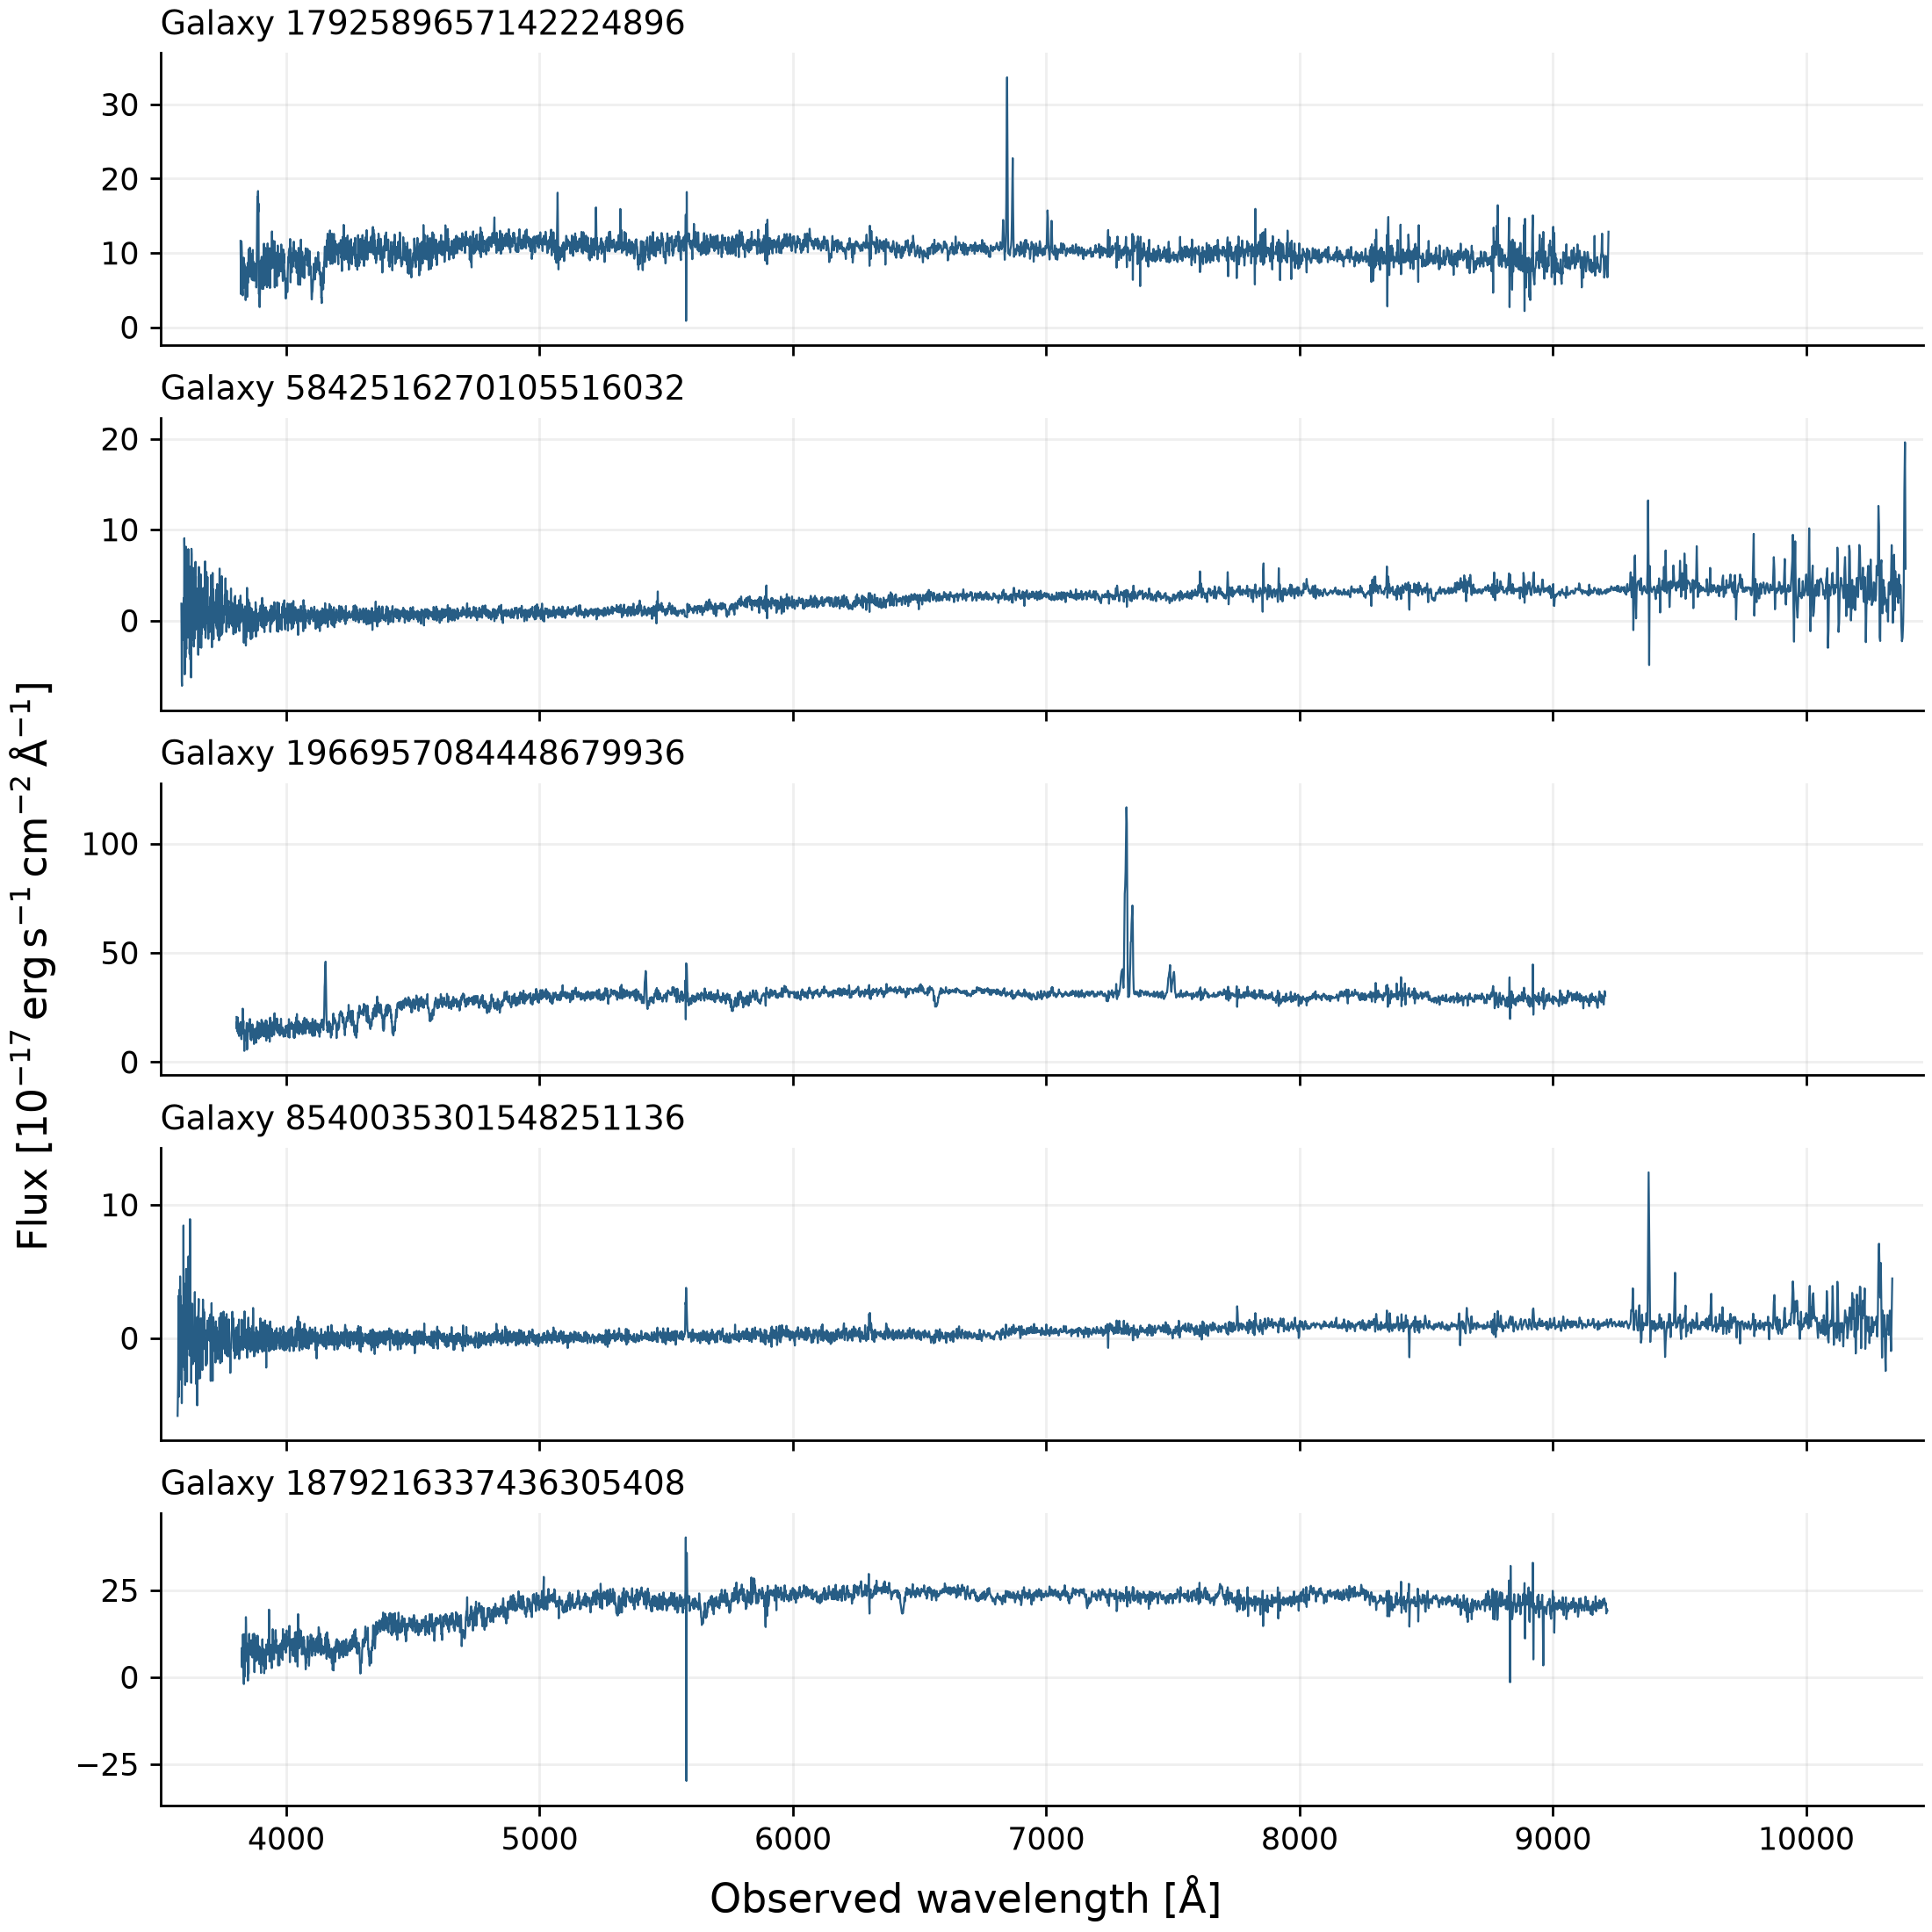
\includegraphics[width=\textwidth]{build/example_galaxy_spectra.png}
\caption{Native spectra of the first five galaxies in the downloaded catalog, before quality filtering or imputation. Each panel shows flux against observed wavelength and uses its own vertical scale.}
\label{fig:example-galaxy-spectra}
\end{figure}

SDSS stores the flux measurement uncertainty as inverse variance, \texttt{ivar}:
\begin{equation}
    \mathrm{ivar}_i = \frac{1}{\sigma_i^2}.
\end{equation}
For positive inverse variance, the variance and standard uncertainty are
\begin{equation}
    \sigma_i^2 = \frac{1}{\mathrm{ivar}_i},
    \qquad
    \sigma_i = \frac{1}{\sqrt{\mathrm{ivar}_i}}.
\end{equation}
I appended these as \texttt{flux\_variance} and \texttt{flux\_uncertainty}. An inverse variance of zero marks an unusable measurement. The quality masks will be dealt with during data preparation.\footnote{SDSS spectral pixel quality flags (SPPIXMASK): \url{https://www.sdss4.org/dr17/algorithms/bitmasks/}.}

\begin{table}[htbp]
\centering
\caption{Spectrum of galaxy \texttt{1792589657142224896} (3828 pixels).}
\label{tab:spectrum-one}
\begingroup
\footnotesize
\setlength{\tabcolsep}{3pt}
\begin{tabular}{rrrrrrrrr}
\toprule
Pixel & \texttt{loglam} & $\lambda$ (\AA) & Flux & \texttt{ivar} & $\sigma^2$ & $\sigma$ & AND & OR \\
\midrule
1 & 3.5820 & 3819.443 & 11.626 & 0.236193 & 4.234 & 2.058 & 0 & 0 \\
2 & 3.5821 & 3820.322 & 8.731 & 0.253389 & 3.947 & 1.987 & 0 & 0 \\
3 & 3.5822 & 3821.202 & 4.456 & 0.270474 & 3.697 & 1.923 & 0 & 0 \\
4 & 3.5823 & 3822.082 & 8.515 & 0.267146 & 3.743 & 1.935 & 0 & 0 \\
$\vdots$ & $\vdots$ & $\vdots$ & $\vdots$ & $\vdots$ & $\vdots$ & $\vdots$ & $\vdots$ & $\vdots$ \\
3825 & 3.9644 & 9212.978 & 8.160 & 0.756741 & 1.321 & 1.150 & 0 & 0 \\
3826 & 3.9645 & 9215.098 & 6.721 & 0.693161 & 1.443 & 1.201 & 0 & 0 \\
3827 & 3.9646 & 9217.223 & 8.531 & 0.614556 & 1.627 & 1.276 & 0 & 0 \\
3828 & 3.9647 & 9219.343 & 12.865 & 0.543218 & 1.841 & 1.357 & 0 & 0 \\
\bottomrule
\end{tabular}
\endgroup
\end{table}

\begin{table}[htbp]
\centering
\caption{Spectrum of galaxy \texttt{5842516270105516032} (4622 pixels).}
\label{tab:spectrum-two}
\begingroup
\footnotesize
\setlength{\tabcolsep}{3pt}
\begin{tabular}{rrrrrrrrr}
\toprule
Pixel & \texttt{loglam} & $\lambda$ (\AA) & Flux & \texttt{ivar} & $\sigma^2$ & $\sigma$ & AND & OR \\
\midrule
1 & 3.5546 & 3585.915 & 1.867 & 0.047831 & 20.907 & 4.572 & 0 & 0 \\
2 & 3.5547 & 3586.740 & -1.194 & 0.063915 & 15.646 & 3.955 & 0 & 0 \\
3 & 3.5548 & 3587.567 & -6.709 & 0.074416 & 13.438 & 3.666 & 0 & 0 \\
4 & 3.5549 & 3588.392 & -7.181 & 0.076003 & 13.157 & 3.627 & 0 & 0 \\
$\vdots$ & $\vdots$ & $\vdots$ & $\vdots$ & $\vdots$ & $\vdots$ & $\vdots$ & $\vdots$ & $\vdots$ \\
4619 & 4.0164 & 10384.841 & 3.687 & 0.007444 & 134.341 & 11.591 & 0 & 167772160 \\
4620 & 4.0165 & 10387.236 & 14.299 & 0.006479 & 154.341 & 12.423 & 0 & 167772160 \\
4621 & 4.0166 & 10389.631 & 19.611 & 0.023951 & 41.752 & 6.462 & 0 & 167772160 \\
4622 & 4.0167 & 10392.016 & 5.706 & 0.104807 & 9.541 & 3.089 & 0 & 0 \\
\bottomrule
\end{tabular}
\endgroup
\end{table}

\clearpage
\section{Data Preparation}

By selecting galaxies with valid catalog target values, I have already handled missing or invalid prediction targets.

There are two options for preparing the spectra. The first is to use the union of all galaxies' wavelength ranges and fill unmeasured flux values with zero, accompanied by an indicator distinguishing missing instrument coverage from a measured zero. The simpler option is to use the intersection of the spectra, retaining only the wavelength range shared by every galaxy.

Based on the spectra investigated so far, the intersection is not much shorter than the average individual spectrum, so I will use this option. I will arrange the shared wavelength centres in ascending order, from the largest starting wavelength to the smallest ending wavelength across the galaxies.

I used the intersection wavelength interval $4416.72\,\text{\AA} \leq \lambda \leq 6848.57\,\text{\AA}$, obtained from the largest starting wavelength and the smallest ending wavelength across all 5,000 galaxies.

For each spectral pixel, the OR mask records quality flags present in at least one exposure, whereas the AND mask records flags present in every exposure.\footnote{SDSS mask interpretation: \url{https://www.sdss4.org/dr17/spectro/spectro_basics/}.} Nonzero masks affect approximately 41\% of pixels in the spectra checked so far. I exclude measurements with chosen AND flags based on ChatGPT's advice interpreting the descriptions of these flags. The selected flags and their descriptions are listed in Appendix~\ref{app:and-flags}. An OR flag can arise from a problem in only some exposures, so I do not exclude measurements on that basis alone. Excluding measurements with the chosen AND flags leaves gaps in the spectra.

I also exclude measurements with NaN or infinite flux or inverse variance, and those with zero or negative inverse variance. This rejects measurements with undefined, zero, or infinite standard uncertainty. Finite, positive uncertainties are retained even when their values are unusually high or low.

Using these criteria, I excluded 1,742,137 of the 21,851,844 flux measurements across all 5,000 native spectra (7.97\%). Within the shared wavelength interval, I excluded 183,048 of 9,530,000 measurements (1.92\%).

To deal with the gaps in the spectra, I exclude galaxies with 10\% or more pixels missing within the shared wavelength range. I then remove wavelength columns with missing measurements in more than 50\% of the training galaxies. This leaves fewer gaps, which I fill using the median of the valid flux measurements at the same wavelength from the training galaxies. These replacements introduce additional uncertainty and may affect the regression and other machine-learning results, but I consider this a good compromise to retain more data.

I discarded 201 of the 5,000 galaxies (4.02\%) because they had 10\% or more pixels missing within the shared wavelength range. I therefore work with 4,799 galaxies.

Figure~\ref{fig:prepared-targets} shows the target values for the prepared spectra.
\begin{figure}[htbp]
\centering
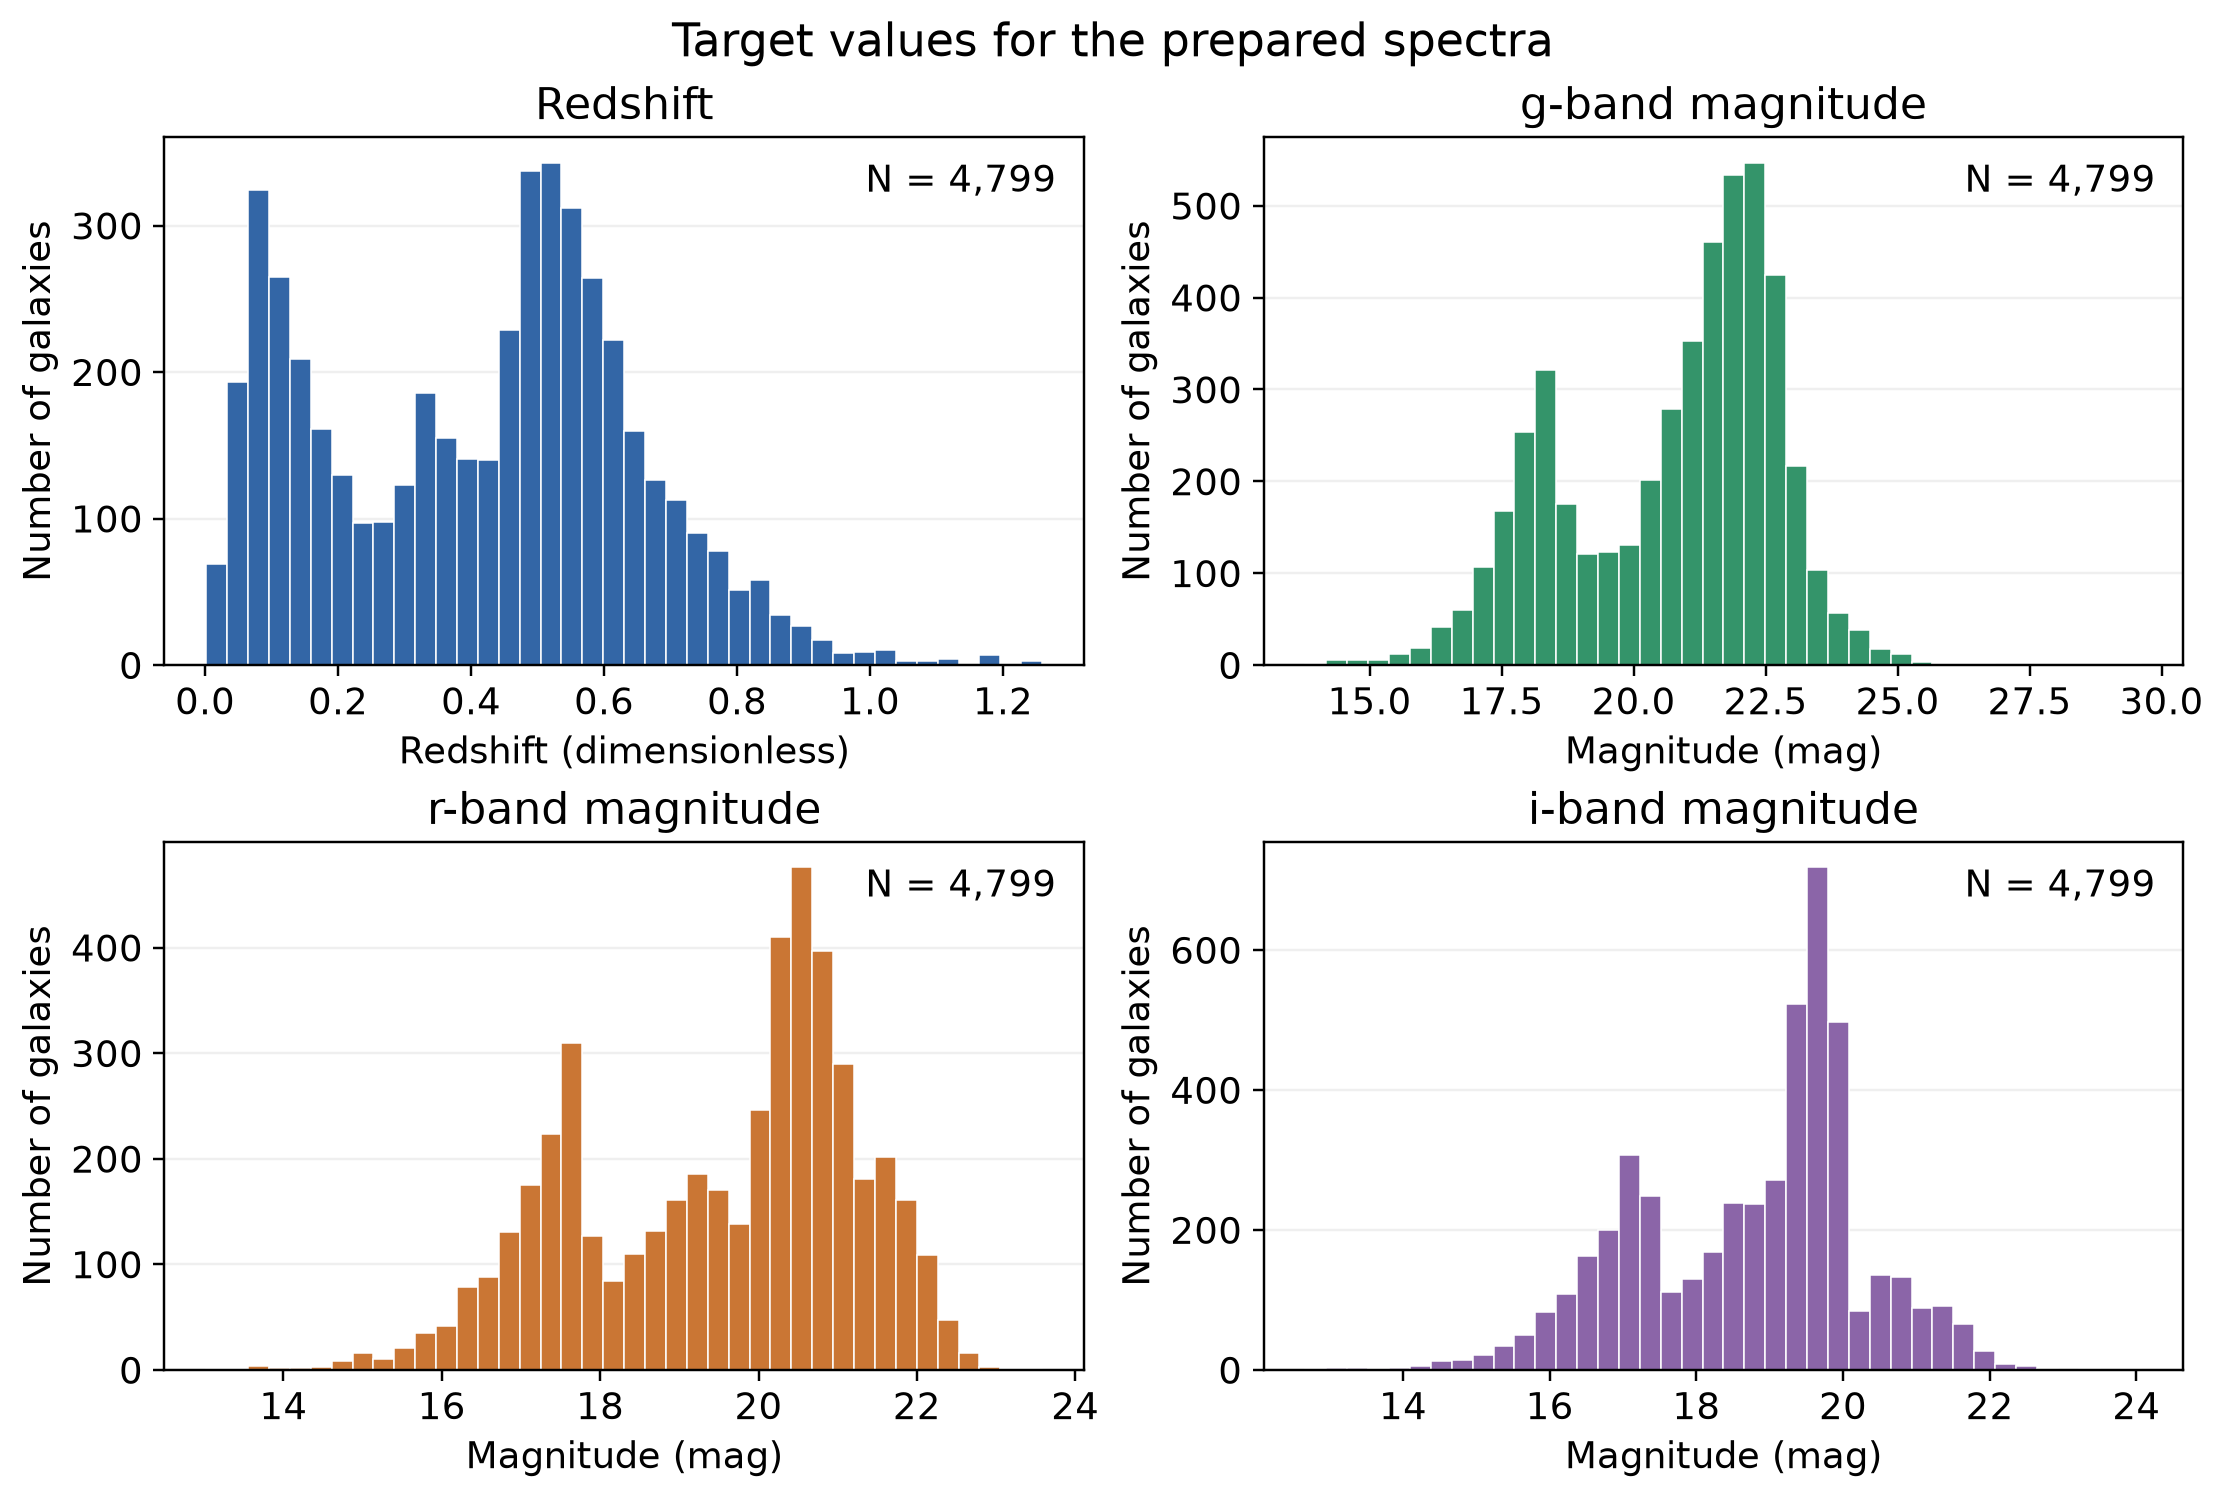
\includegraphics[width=\textwidth]{build/prepared_target_distributions.png}
\caption{Target values for the prepared spectra of the 4,799 retained galaxies.}
\label{fig:prepared-targets}
\end{figure}

\clearpage
\section{Linear Regression}

\subsubsection{Performing the Linear Regression}

I perform the linear regression using scikit-learn.\footnote{\raggedright scikit-learn LinearRegression documentation: \url{https://scikit-learn.org/stable/modules/generated/sklearn.linear_model.LinearRegression.html}.} I have prepared the data as explained in the previous sections to give me the inputs for all four targets. I ended up with 1,902 flux values per galaxy and 815 missing-values which I have filled with the medians, giving me $p=2,717$ input values. I predict each target using the following equation:
\begin{equation}
    \hat y_i = b + \omega_1 x_{1i} + \cdots + \omega_p x_{pi}.
\end{equation}
The target $y$ can be redshift or the magnitude in the $g$, $r$, or $i$ band, with a separate model fitted for each. Here, $\hat y_i$ is the predicted value for galaxy $i$, $b$ is the intercept, $\omega_j$ are the weights, and $x_{ji}$ are the input data. The intercept and weights are fitted during training.

Scikit-learn minimizes the sum of squared errors:
\begin{equation}
    \min_{b,\mathbf w}\sum_{i=1}^{N}(y_i-\hat y_i)^2,
    \qquad \mathbf w=(\omega_1,\ldots,\omega_p),
\end{equation}
where $y_i$ is the actual catalog value and $N$ is the number of training galaxies. It does this using a numerical linear-algebra solver.

\subsubsection{Validation}

I am using mean absolute error (MAE), which is the metric that measures the average absolute distance between a prediction and the actual value:
\begin{equation}
    \mathrm{MAE}=\frac{1}{N}\sum_{i=1}^{N}|y_i-\hat y_i|.
\end{equation}

\begin{table}[htbp]
\centering
\small
\setlength{\tabcolsep}{3pt}
\caption{Validation MAE and training times for the four targets. Training is timed for one fit. Loading and saving are excluded.}
\begin{tabular}{lrlr}
\toprule
Target & MAE & Unit & \shortstack{Training\\(s)} \\
\midrule
Redshift ($z$) & 0.241816 & Dimensionless & 6.703 \\
$g$-band magnitude & 1.533109 & mag & 6.109 \\
$r$-band magnitude & 1.251973 & mag & 6.094 \\
$i$-band magnitude & 1.168410 & mag & 6.885 \\
\bottomrule
\end{tabular}
\end{table}

As shown in Figure~\ref{fig:prepared-targets}, this method did not work well for redshift, since the values are generally between 0 and 1 and the MAE is approximately 0.242. For the magnitudes, which are usually between 14 and 24~mag, the MAE is approximately 1.17--1.53~mag. Since magnitudes use a logarithmic scale, these errors are substantial as well.\footnote{SDSS magnitude definitions: \url{https://www.sdss4.org/dr17/algorithms/magnitudes/}.}

\clearpage
\section{Random Forest Regressor}

\subsubsection{Performing the Random Forest Regression}

I perform the random forest regression using scikit-learn as well.\footnote{\raggedright scikit-learn RandomForestRegressor documentation: \url{https://scikit-learn.org/stable/modules/generated/sklearn.ensemble.RandomForestRegressor.html}.} I set the number of trees using \texttt{n\_estimators}, which controls how many trees form the forest. According to the scikit-learn guidance, more trees usually improve the results, but at some point the improvements flatten out while the computation time increases.\footnote{\raggedright scikit-learn guidance on random forest parameters: \url{https://scikit-learn.org/stable/modules/ensemble.html\#parameters}.} I started from the default value of 100 trees and also tried 200 and 400.

A tree is built by choosing a sample of objects, in this case galaxies, with replacement, so some galaxies can appear more than once. Their features are then investigated to split them into groups. At each node, the algorithm randomly chooses a portion of the features to consider. I started from the default \texttt{max\_features} value of 1.0, meaning all features, and also tried 0.5 and 0.3, meaning 50\% and 30\% of the features.

For the chosen features, the algorithm tries different thresholds, splitting the group according to whether a feature value is below or above a threshold. It chooses the single feature and threshold that minimize the sum of squared distances between the resulting groups' target values and their respective target averages. The process then repeats within each group.\footnote{\raggedright scikit-learn decision tree splitting and regression criteria: \url{https://scikit-learn.org/stable/modules/tree.html\#mathematical-formulation}.}

I control how small the final groups can become using \texttt{min\_samples\_leaf}. I started from the default value of 1 and also tried 3, 5, and 10. A split is allowed only if both resulting groups contain at least this many training samples. The maximum tree depth remains unrestricted. Each final group is a leaf, whose prediction is the average target value of its training galaxies.

These trees form the forest. To make a prediction, I send a test galaxy through each tree and take the mean of their predictions.

My method was to try the different forest sizes, choose the one with the best validation MAE, and fix it. I then chose the best feature percentage by MAE with the tree count fixed. Finally, I fixed those two parameters and looked for the best minimum leaf size. I did this separately for all four targets. These parameters are interdependent, so to look for better results I could have tried every combination of the tested values. However, since I obtained sufficient results this way, I keep this strategy. Table~\ref{tab:rf-tuning} shows the validation MAE for every tested value and target.

I chose 400 trees and 30\% of the features for redshift, 200 trees and 30\% for the $g$-band magnitude, 200 trees and 100\% for the $r$-band magnitude, and 400 trees and 100\% for the $i$-band magnitude. I chose a minimum leaf size of 1 for all four targets.

\begin{table}[p]
\centering
\caption{Validation MAE for every random forest parameter combination. Rows correspond to targets and columns to the three parameters. The filled point marks the lowest MAE in each plot.}
\label{tab:rf-tuning}
\begingroup
\small
\setlength{\tabcolsep}{2pt}
\begin{tabular}{@{}lccc@{}}
\toprule
Target & Number of trees & Features (\%) & Minimum leaf size \\
\midrule
Redshift &
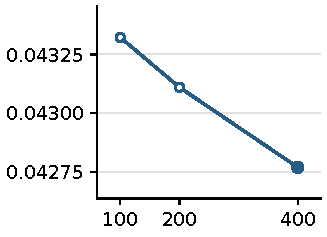
\includegraphics[width=0.285\textwidth]{build/rf_mae_z_trees.pdf} &
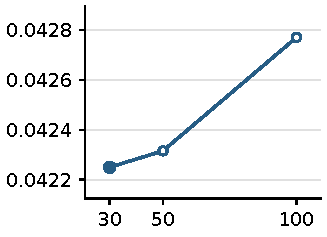
\includegraphics[width=0.285\textwidth]{build/rf_mae_z_features.pdf} &
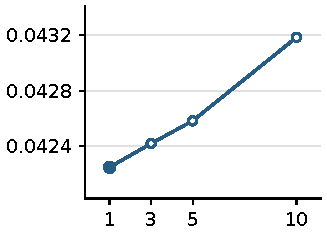
\includegraphics[width=0.285\textwidth]{build/rf_mae_z_leaves.pdf} \\
$g$ band &
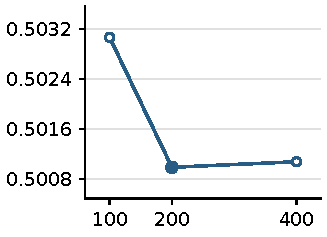
\includegraphics[width=0.285\textwidth]{build/rf_mae_cModelMag_g_trees.pdf} &
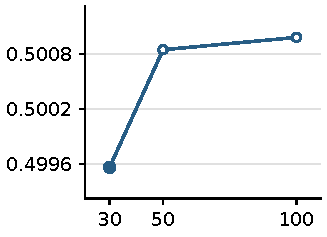
\includegraphics[width=0.285\textwidth]{build/rf_mae_cModelMag_g_features.pdf} &
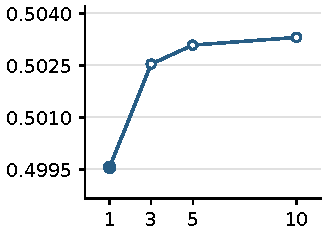
\includegraphics[width=0.285\textwidth]{build/rf_mae_cModelMag_g_leaves.pdf} \\
$r$ band &
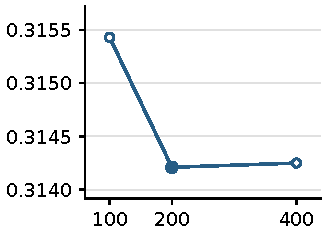
\includegraphics[width=0.285\textwidth]{build/rf_mae_cModelMag_r_trees.pdf} &
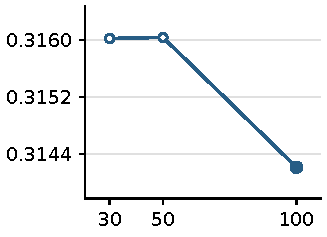
\includegraphics[width=0.285\textwidth]{build/rf_mae_cModelMag_r_features.pdf} &
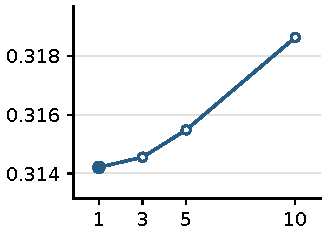
\includegraphics[width=0.285\textwidth]{build/rf_mae_cModelMag_r_leaves.pdf} \\
$i$ band &
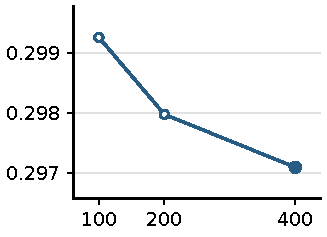
\includegraphics[width=0.285\textwidth]{build/rf_mae_cModelMag_i_trees.pdf} &
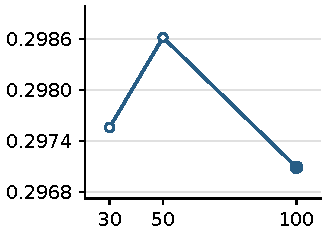
\includegraphics[width=0.285\textwidth]{build/rf_mae_cModelMag_i_features.pdf} &
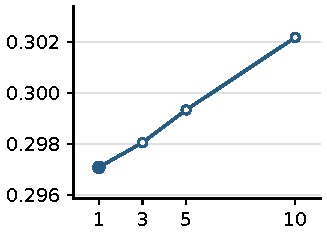
\includegraphics[width=0.285\textwidth]{build/rf_mae_cModelMag_i_leaves.pdf} \\
\bottomrule
\end{tabular}
\endgroup
\end{table}

\clearpage
\subsubsection{Validation}

Validating the same way I did before:

\begin{table}[htbp]
\centering
\small
\setlength{\tabcolsep}{3pt}
\caption{Random forest validation MAE for the four targets.}
\label{tab:rf-validation}
\begin{tabular}{lrlr}
\toprule
Target & MAE & Unit & \shortstack{Training\\(s)} \\
\midrule
Redshift ($z$) & 0.042249 & Dimensionless & 60.410 \\
$g$-band magnitude & 0.499563 & mag & 33.043 \\
$r$-band magnitude & 0.314209 & mag & 110.882 \\
$i$-band magnitude & 0.297089 & mag & 240.538 \\
\bottomrule
\end{tabular}
\end{table}

It can be seen that the results are a magnitude better than with linear regression.

\clearpage
\section{Principal Component Analysis}

I can capture the variance in the data with principal component analysis (PCA). Using scikit-learn, I form weighted sums of the centred features along linearly independent directions.\footnote{\raggedright scikit-learn PCA documentation: \url{https://scikit-learn.org/stable/modules/generated/sklearn.decomposition.PCA.html}.} Performing PCA gives 92.71\% of the training variance encoded in the first component and 5.09\% in the second. With these two, 97.80\% of the training variance is maintained. PCA preparation takes 4.581~s to fit and 0.0306~s to transform the training and validation galaxies; the regression timings below exclude this shared cost. Figure~\ref{fig:pca-galaxies} shows the galaxies in the coordinate system of these two components.

\begin{figure}[htbp]
\centering
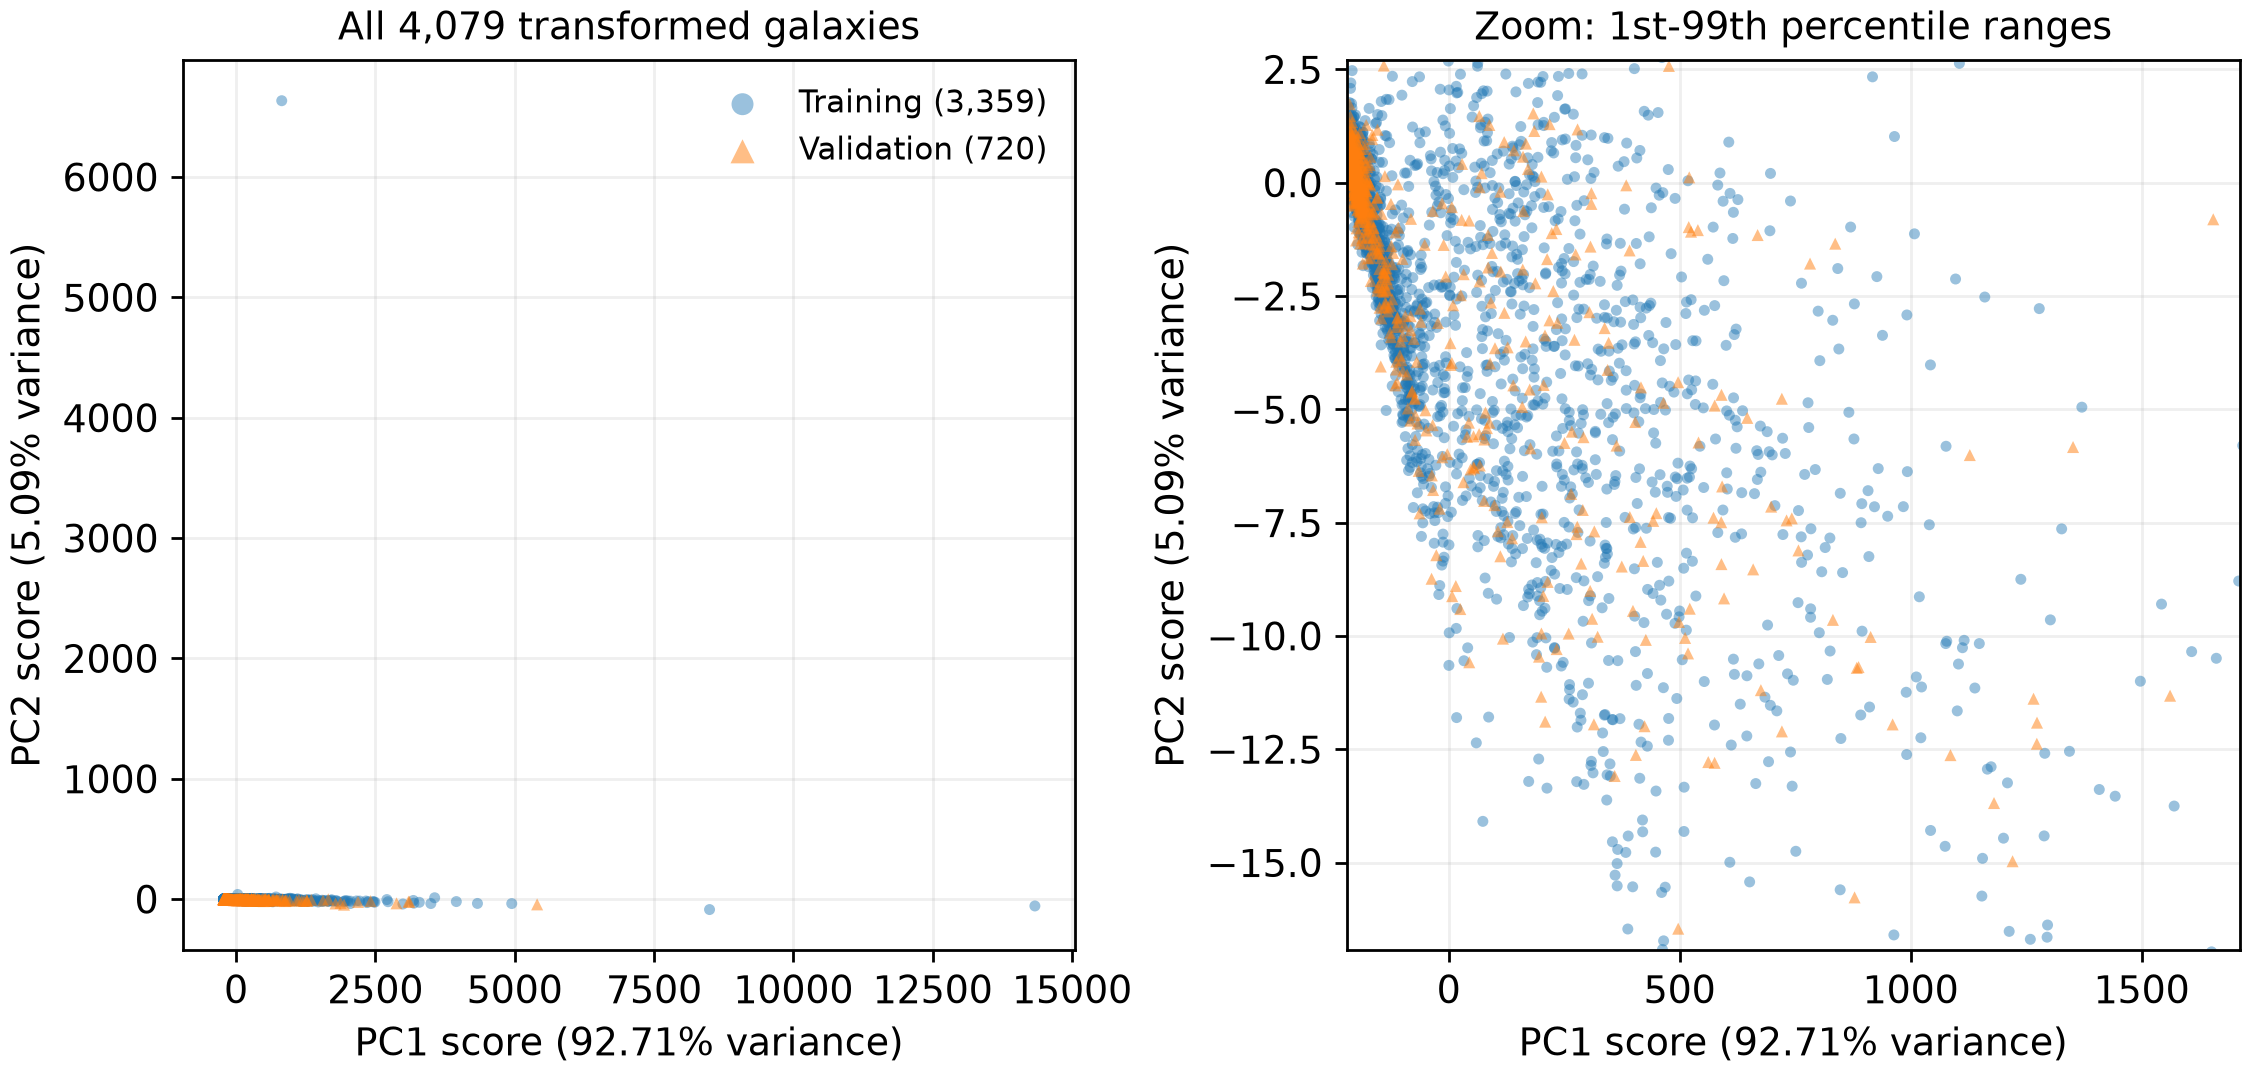
\includegraphics[width=\textwidth]{build/pca_galaxy_projection.png}
\caption{Coordinates of the 3,359 training and 720 validation galaxies along the first two principal components. PCA was fitted using the training galaxies only. The left panel shows the full range; the right panel zooms to the 1st--99th percentile range of each coordinate.}
\label{fig:pca-galaxies}
\end{figure}

\clearpage
\subsection{Performing the Machine Learning Regression on the New Feature Basis}

I can perform the previous machine learning methods with these two principal components as two features. The methods have already been described, so I will just show the results. I use the same training and validation galaxies as before. The percentage changes compare each model's MAE with its earlier result; negative values mean an improvement and positive values mean a worse result.

\subsubsection{Linear Regression on the Two Principal Components}

\begin{table}[htbp]
\centering
\small
\setlength{\tabcolsep}{3pt}
\caption{Validation MAE for linear regression on the two principal components, compared with the earlier linear regression.}
\label{tab:pca-linear-validation}
\begin{tabular}{lrrrlr}
\toprule
Target & MAE & \shortstack{Earlier\\MAE} & \shortstack{Change\\(\%)} & Unit & \shortstack{Training\\(s)} \\
\midrule
Redshift ($z$) & 0.154425 & 0.241816 & $-36.1$ & Dimensionless & 0.0017 \\
$g$-band magnitude & 1.133543 & 1.533109 & $-26.1$ & mag & 0.0020 \\
$r$-band magnitude & 1.035589 & 1.251973 & $-17.3$ & mag & 0.0017 \\
$i$-band magnitude & 0.870112 & 1.168410 & $-25.5$ & mag & 0.0019 \\
\bottomrule
\end{tabular}
\end{table}

With the two principal components, the linear regression performs better for all four targets, with MAE reductions of approximately 17--36\%.

Excluding PCA preparation, training is approximately 3,948, 3,125, 3,536, and 3,551 times faster for redshift and the $g$, $r$, and $i$ magnitudes, respectively, than with the original inputs.

\subsubsection{Random Forest Regressor on the Two PCA Components}

I keep the previously chosen random forest parameters for each target.

\begin{table}[htbp]
\centering
\small
\setlength{\tabcolsep}{3pt}
\caption{Validation MAE for the random forest regressor on the two principal components, compared with the earlier random forest regressor.}
\label{tab:pca-forest-validation}
\begin{tabular}{lrrrlr}
\toprule
Target & MAE & \shortstack{Earlier\\MAE} & \shortstack{Change\\(\%)} & Unit & \shortstack{Training\\(s)} \\
\midrule
Redshift ($z$) & 0.060114 & 0.042249 & $+42.3$ & Dimensionless & 0.496 \\
$g$-band magnitude & 0.551575 & 0.499563 & $+10.4$ & mag & 0.241 \\
$r$-band magnitude & 0.377780 & 0.314209 & $+20.2$ & mag & 0.261 \\
$i$-band magnitude & 0.389588 & 0.297089 & $+31.1$ & mag & 0.491 \\
\bottomrule
\end{tabular}
\end{table}

With the two principal components, the random forest regressor performs worse for all four targets, with MAE increases of approximately 10--42\%.

Excluding PCA preparation, training is approximately 121.9, 137.3, 424.8, and 489.4 times faster for redshift and the $g$, $r$, and $i$ magnitudes, respectively, than with the original inputs.

\clearpage
\subsubsection{Random Forest Regressor with optimized parameters}

I repeat the parameter testing on the two principal components, using the same sequence as before: 100, 200, and 400 trees; 100\%, 50\%, and 30\% of the features; and minimum leaf sizes of 1, 3, 5, and 10. With two features, both 50\% and 30\% select one feature per split.

\begin{table}[htbp]
\centering
\small
\setlength{\tabcolsep}{3pt}
\caption{Selected parameters and validation MAE after retuning the random forest on PC1 and PC2. The reduction is relative to the two-component forest with the earlier parameters.}
\label{tab:pca-retuned-forest}
\begin{tabular}{lrrrrrr}
\toprule
Target & Trees & \shortstack{Features\\(\%)} & \shortstack{Leaf\\size} & MAE & \shortstack{Reduction\\(\%)} & \shortstack{Training\\(s)} \\
\midrule
Redshift ($z$) & 100 & 50 & 10 & 0.056800 & 5.5 & 0.111 \\
$g$-band magnitude & 200 & 30 & 10 & 0.524210 & 5.0 & 0.212 \\
$r$-band magnitude & 200 & 50 & 10 & 0.349716 & 7.4 & 0.221 \\
$i$-band magnitude & 400 & 50 & 10 & 0.359487 & 7.7 & 0.416 \\
\bottomrule
\end{tabular}
\end{table}


Excluding PCA preparation and parameter testing, training is approximately 545.2, 155.5, 501.2, and 578.6 times faster for redshift and the $g$, $r$, and $i$ magnitudes, respectively, than with the original inputs. Compared with the two-component forest before retuning, training is 4.5, 1.1, 1.2, and 1.2 times faster for the same targets, respectively.

\clearpage
\section{Discussion}

PCA reduced the model training times substantially, as I expected and as shown in the tables. For linear regression, the model gave better predictions when it learned on the principal components. This was counterintuitive to me: my first instinct was that every machine learning algorithm should perform worse when information is excluded from the dataset.

To understand this, I consulted ChatGPT. My current understanding is that small fluctuations in strongly correlated neighbouring spectral values can lead to large, opposing fitted weights, making the model overfit the training data. Retaining only two principal components may have reduced this effect.

The random forest regressor seemed to be adversely affected by excluding this information and reducing the available features to two.

\clearpage
\appendix
\section{Selected AND Flags}
\label{app:and-flags}

The following flags were selected for exclusion based on ChatGPT's recommendation of the SDSS SPPIXMASK descriptions.\footnote{SDSS SPPIXMASK definitions: \url{https://www.sdss4.org/dr17/algorithms/bitmasks/}.}

\begin{table}[htbp]
\centering
\small
\begin{tabular}{@{}p{4.2cm}p{10.8cm}@{}}
\toprule
Flag & Brief description \\
\midrule
\texttt{NOPLUG} & The fiber is absent from the mapping of plugged fibers. \\
\texttt{BADTRACE} & The estimated path of the spectrum on the detector is unreliable. \\
\texttt{BADFLAT} & The fiber's flat-field exposure has low counts. \\
\texttt{BADARC} & The arc-based wavelength calibration is unreliable. \\
\texttt{MANYBADCOLUMNS} & Bad detector columns affect over 10\% of pixels. \\
\texttt{MANYREJECTED} & Extraction rejects over 10\% of pixels. \\
\texttt{LARGESHIFT} & The object and flat-field positions differ substantially. \\
\texttt{BADSKYFIBER} & A sky fiber has unusually large residuals. \\
\texttt{LOWFLAT} & The flat-field response falls below 0.5. \\
\texttt{FULLREJECT} & Extraction rejects the pixel completely. \\
\texttt{SCATTEREDLIGHT} & Scattered light makes a significant contribution. \\
\texttt{CROSSTALK} & Contamination from other spectra is significant. \\
\texttt{NOSKY} & The sky background cannot be determined at this wavelength. \\
\texttt{BRIGHTSKY} & The sky signal exceeds the pipeline's brightness thresholds. \\
\texttt{BADFLUXFACTOR} & The calibration or correction factor for flux is low. \\
\texttt{BADSKYCHI} & Sky residuals have relative $\chi^2$ above 3. \\
\texttt{REDMONSTER} & A contiguous wavelength region has excessive sky-residual $\chi^2$. \\
\bottomrule
\end{tabular}
\end{table}

\clearpage
\section*{AI Usage Statement}

I used OpenAI's Codex AI assistant through the Codex interface in Visual Studio Code for coding and writing assistance with model \texttt{gpt-6.1-sol}. References to ChatGPT elsewhere in the report describe the conversational explanations provided by the assistant.

Coding assistance was substantial: the assistant generated, revised, debugged and executed notebook cells and supporting Python scripts. This covered the SQL query and spectrum downloads, FITS inspection, wavelength alignment, mask filtering, missing-value handling, training/validation/test splits, linear regression, random forests, parameter searches, PCA, plots, MAE tables and runtime measurements. It also helped set up the Python environment and background execution. The numerical results were obtained by running the analysis code on the SDSS data.

I also used the assistant to understand astronomical quantities and machine-learning methods and to discuss methodological choices. AI recommendations influenced the sample size of 5,000 galaxies, selected mask exclusions, missing-data policy and model settings. 

For writing, I supplied instructions and draft wording through the conversation. It did not start as me just drafting the sentences, but while I wanted to write stuff like 'badly affected' it corrected it to 'adversely affected' which I did not read enough to say on my own and this way it sound way better. I am working on it though reading Children of time big time. The assistant drafted and revised parts of the English report, corrected language, typeset equations, I asked it to insert the relevant citations and computed tables, and formatted and compiled the LaTeX document. The discussion was written from my stated interpretation, informed by AI explanations. I remain responsible for the final submitted code, text and interpretation.

The project files, prepared data and notebook are available in the \href{https://github.com/malkouka07/Data_mining_machine_learning_course/tree/main/SDSS-spectral-analysis}{GitHub repository}.

\end{document}
